%!TEX root = ../BPlusTree-report.tex
\section{Background}
\label{sec:Background}
% Notes:
% What is a bplustree:
%   - Inherently imperative data structure
%   - Suboptimal implementation
%     - Running time of optimal implementation
%     - Running time of our implementation
%       - Mention how one could make it optimal.
%       - A tree in a tree in a tree, dawg
%     - Running time out of scope
\label{subsec:Background_Bplus_tree}
The B+ tree is a n-ary, self-balancing, tree data structure\,\cite[pp. 334]{ramakrishnan2003database}, similar to a B-tree. It is composed of nodes, leaves and a root, which can be either a node or a leaf. Nodes hold keys and pointers, and leaves hold keys mapped to values, as shown in Fig. \ref{fig:bplustree}. Duplicate keys are not allowed. A pointer $p_0$ in a node points to the subtree containing keys with values lower than the key $k$ following $p_0$. The next pointer in the node, $p_1$ points to the subtree containing keys with values that are larger than $k$. For a given B+ tree, an order, $b$, determines the capacity of nodes and leaves\,\cite[p. 335]{ramakrishnan2003database}. See Table \ref{tab:bpluschildren} for capacities. In most B+ tree implementations, each leaf is joined to the next leaf by a pointer, allowing fast sequential access to values, which is useful for range queries.

% Maybe use this $\forall~k_0\in p_0,~k_1\in p_1: k_0< k < k_1$

\begin{figure}
 \centering
   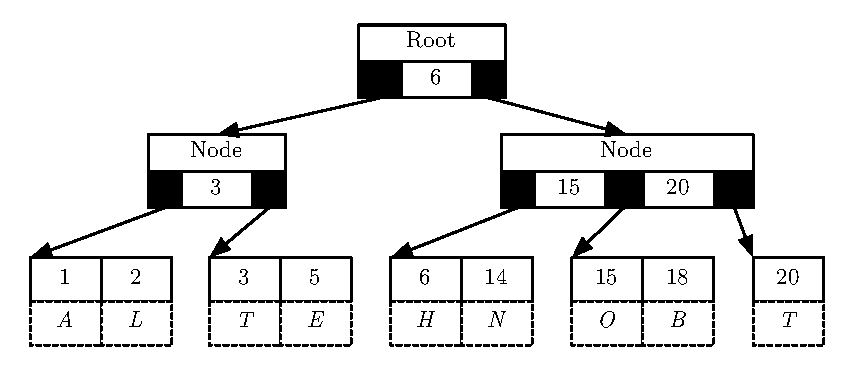
\includegraphics[width=90mm]{diagrams/BPlusTree.pdf}
 \caption{An example of a B+ tree with $b=1$. The black boxes in the root and nodes are pointers to subtrees. The bottom row contains leaves, with values, in this case characters, in the dashed boxes. Pointers connect the leaves.}
 \label{fig:bplustree}
\end{figure}

\begin{table}
\centering
\label{tab:bpluschildren}
\begin{tabular}{| l | l | l | l | l | }
\hline
           & Min keys~ & Max keys~ & Min children~ & Max children~ \\ \hline
Root node~ &  1  & $2b$ &  2    & $2b+1$ \\ \hline
Root leaf  &  0  & $2b$ &  0    & $2b$   \\ \hline
Node       & $b$ & $2b$ & $b+1$ & $2b+1$ \\ \hline
Leaf       & $b$ & $2b$ & $b$   & $2b$   \\ \hline
\end{tabular}
\caption{Capacity of nodes and leaves in a B+ tree.}
\end{table}

\paragraph{}
In this project, we will work with three functions, which we will refer to as our primary functions. These are: $insert$, $search$ and $height$. The theory behind the $height$ function is trivial, as a B+ tree is always balanced, and will not be explained in this section, but the theory behind the $insert$ and $search$ functions require some explanation. The deletion function is beyond the scope of this project, as the work required for just the $insert$ and $search$ functions is substantial.

\subsubsection{Search}
\label{subsec:Search}
The $search$ function takes two arguments: a search key $sk$, and a tree, $t$, to search in. The tree can be either a node or a leaf. If the tree is a node, the function finds the pointer $p$ in the node for which it holds that:
\begin{itemize}
	\item $p$ is the first pointer in the node, and there exists a key $k$ that immediately succeeds $p$, where $sk < k$ OR
	\item The keys $k_1$ and $k_2$ exist on either side of $p$, such that $k_1 \le sk < k_2$ OR
	\item $p$ is the last pointer in the node, and for all keys $k$ in the node $k \le sk$.
\end{itemize}
The function then recursively calls itself with the subtree $p$. Once the function reaches a leaf, it searches for the key, often with a binary search in an array or tree. The function then returns the found value. This results in a time complexity of $O(h~log(b))$, as one node in each level must be visited, and the binary search takes $log(b)$ operations.

\subsubsection{Insert}
The $insert$ function takes two arguments: a key-value pair $(k, v)$ and a tree $t$ to insert the pair into. The function starts at the root of the tree, and recursively searches for the leaf to insert into. It does this search in the same way the $search$ function does. The pair is then inserted into the leaf at the correct position. If the insertion results in the leaf having more than $2b$ values, the leaf must be split. This is called a leaf overflow. This is handled by splitting the leaf in half, and inserting a pointer to the new leaf in the parent node. If the parent node now has more than $2b+1$ children, it must also be split, following the same pattern. This can continue all the way to the root, which in turn can be split into two subtrees. If this happens, a new root node is created, and the two subtrees from the split of the previous root are inserted as children. After the root has been split, the height of the tree has increased by one. Thus, a B+ tree can be seen to grow up from the leaves, and is always in balance. The complexity of such an $insert$ function is $O(h~log(b))$, using the same reasoning as for search, and assuming that nodes and leaves with overflows can be split in constant time.
